\documentclass{ametsoc}
\usepackage[]{graphicx}
\usepackage{alltt}
\usepackage{siunitx}
%
%==============================================================================
\journal{jcli}

%
%==============================================================================
\bibpunct{(}{)}{;}{a}{}{,}

\title{Effects of Natural Variability of Seawater Temperature, Time Series Length, Decadal Trend, and Instrument Precision on the Ability to Detect Temperature Trends}

\authors{Robert Schlegel\correspondingauthor{Robert Schlegel, Department of Biodiversity and Conservation Biology, University of the Western Cape, Bellville, Republic of South Africa.}
 and Albertus Smit}

\affiliation{Department of Biodiversity and Conservation Biology, University of the Western Cape, Bellville, Republic of South Africa}

\email{wiederweiter@gmail.com}

%
%==============================================================================
\abstract{In South Africa 129 \emph{in situ} temperature time series of 1 to 43 years are used for investigations of the thermal characteristics of coastal seawater. They are comprised of temperature recordings at precisions ranging from \SIrange{0.5}{0.001}{\degreeCelsius} and collected with handheld thermometers or underwater temperature recorders (UTRs). Using the naturally occurring range of seasonal signals, variability and temperature trends for 84 of these time series, the length, decadal trend and data precision of each time series were systematically varied before fitting generalized least squares (GLS) models to study the effect these variables have on trend detection. We determined that low instrument precision has less effect on the ability of a model to detect trends within a time series than do the length, variance or the decadal trend itself, with length contributing the most to trend detection. We found that time series at least 20 years in length may be used tentatively for climate change research, but that time series >30 years in length are preferable. The implication is that long-running thermometer time series in this dataset, and others around the world, are more useful for decadal scale climate change studies than the shorter, more precise UTR time series.}

% AJS: At the same length, which is most useful: thermometer or UTR recordings?
% RWS: Given everything I've learned of instrument precision and the results of these analyses, I would say they are the same. I was going to say so in the abstract but decided against it. I need to perform an investigation into this by comparing closeness of fit to DT_model and DT with varying length against the different types. I think thermo's may actually be better....

\emph{We need to say something at the end about things we did not study, which may be more important i.t.o. trend detection -- instrumental drift. There is also the aspect of accuracy that can/should be mentioned, and although (given a stable instrument without drift) can yield reliable, useful and precise trend estimates, can nevertheless be off in regards to know the real temperature.}

%==============================================================================
\begin{document}

\maketitle

\section{Introduction}
The roughly ~3,000 km of South Africa's coastline is bordered by the Benguela and Agulhas currents \citep[e.g.][]{Roberts2005,Hutchings2009}, which, in combination with other nearshore processes, affect the country's marine coastal ecosystems \citep{Santos2012a}. A thorough understanding of these coastal processes is provided by several physical variables, of which temperature is one of the main determinants \citep[e.g.][]{Blanchette2008, Tittensor2010, Couce2012}. In order to ensure a true representation of organisms' biological thermal limits, nearshore temperatures must be accurately recorded and monitored. Some sources warn of the pitfalls in doing so \emph{RWS: Add references here showing which sources say using SST for the coast is inappropriate}, and a study by \citet{Smit2013} showed that SST data have a warm bias as large as \SI{6}{\degreeCelsius} when compared to coastal \emph{in situ} data. Nevertheless, a widespread approach in coastal ecological research is to use satellite and/or model-generated temperature data as representation of the sea surface temperature (SST) along coastlines \citep[e.g.][]{Blanchette2008, Broitman2008a, Tyberghein2012}, because apparently the dangers of applying gridded SSTs to the coast are not widely known or in many places in the world there simply are no suitable \emph{in situ} coastal temperature time series available. It is for this reason that we strongly recommended the use of \emph{in situ} data to support research conducted within 400 m from the shoreline.

Where records of \emph{in situ} coastal seawater temperature do exist, the reliability of many of these datasets that could be used in place of the remotely-sensed SST data remains to be verified. Users of SST data benefit from it being refined through a number of well documented validation and quality control processes \citep[e.g.][]{Reynolds1994, Brown1999, Martin2012}, whereas the standards and methods with which local \emph{in situ} data from a single dataset are collected and refined may differ greatly. For example, there are currently seven organizations and/or governmental departments (hereafter referred to as bodies) contributing coastal seawater temperature data to the South African Coastal Temperature Network (SACTN). These bodies use different methods and instruments to collect their data as no national standard has been set. One consequence of this methodological disparity is that two thirds of the data were sampled with hand-held thermometers that are manually recorded at a data precision of \SI{0.5}{\degreeCelsius}, as opposed to the current generation of Underwater Temperature Recorders (UTRs) with an instrument precision of up to \SI{0.001}{\degreeCelsius}. If these \emph{in situ} data are to be used together \emph{in lieu} of the satellite-based SST data, it is important that the characteristics of the contributing data sources are understood in terms of their ability to yield useful, reliable and accurate long-term measurements for use in climate change studies.

This prompted us to examine the 129 \emph{in situ} time series that comprise the SACTN, whose locations and instrument types may be seen in Figure \ref{figure01}. The range of data precision and statistical characteristics found within this dataset were used to guide a series of enquiry-driven analyses into the suitability of the time series to yield statistically significant assessments of decadal temperature change. The length, decadal trend and data precision of each time series were adjusted in a systematic manner, and forms the core of our analyses. Our aim was to assess the effect that each of these variables has on the ability of a model to detect a decadal trend within time series that differ in their decadal trends and variance properties. The effect gaps in the time series may have on the fitting of models was also investigated as many of the time series used here have missing data scattered throughout, which is unavoidable for a 20+ year time series that is sampled by hand by a single technician at each site.

The study provides a better understanding of some of the determinants of a time series that are influential in the detection success of decadal trends in coastal ocean temperature time series.

\section{Methods}

\subsection{Data Sources}
Our study lies within the political borders of South Africa's coastline. The location of each point of collection may be found in Figure \ref{figure01}. Of the 129 time series used, 43 are recorded with UTRs and the other 86 with hand-held mercury thermometers. The oldest currently running time series began on January 1st, 1972; there are 11 total time series that started in the 70s, 53 more started in the 80s, 34 began in the 90s, 18 in the 00s and 13 in the current decade.

The data are collected using two different methods and a variety of instruments. Hand-held mercury thermometers (which are being phased out in favor of alcohol thermometers or electronic instruments) are used in some instances at the shoreline, and represent seawater temperatures at the surface. At other places, predominantly along the country's east coast, data are collected with glass thermometers from a small boat at the location of shark nets along the coast \citep{Cliff1988}. Data at other localities are collected using delayed-mode instruments that are permanently moored shallower than 10 m, but generally very close to the surface below the low-water spring tide level.

Over the last 40+ years the electronic instruments used have changed and improved. The previous standard was the Onset Hobo UTR with a thermal precision of \SI{0.01}{\degreeCelsius}. The meta-data pertaining to these older temperature records and to those that came before, such as the instrumentation used and the motivation behind the levels of precision at which the data were recorded, have over time been lost, highlighting the issues of staff rotation in government departments and the importance of implementing meta-data standards at a very early stage in any monitoring programme. The new standard currently being phased in is the Starmon Mini UTR. These devices have a maximum thermal precision of \SI[separate-uncertainty = true, multi-part-units = repeat]{0.001(25)}{\degreeCelsius} (http://www.star-oddi.com/). Of the 43 UTR time series in this dataset, 30 were recorded at a precision of \SI{0.001}{\degreeCelsius} for their entirety, five UTR time series include older data that were recorded at a precision of \SI{0.01}{\degreeCelsius} or \SI{0.1}{\degreeCelsius} and so have been rounded down to match this level of precision. Eight additional UTR time series have older data that were recorded at a precision of \SI{0.1}{\degreeCelsius}.

% AJS: I would leave this out:
% UTR time series recorded entirely at a precision of \SI{0.001}{\degreeCelsius} are grouped in the `new' subgroup of time series and those with data recorded at lower precisions are grouped in the `old' subgroup. Time series recorded with handheld thermometers have been grouped in the `thermo' subgroup. We provide no information about the accuracy of the temperature recordings.

The thermometer data are recorded manually and saved in an aggregated location at the head offices of the collecting bodies. UTRs are installed and maintained by divers and data are retrieved at least once annually. These data are digital and are downloaded to a hard drive at the respective head offices of the collecting bodies.

\subsection{Data Management}
Each of the seven bodies contributing data to this study have their own method of data formatting. Steps are being taken towards a national standard as we move towards replacing all the thermometer recordings with UTR devices; however, as of the writing of this article, one does not yet exist. Data from each organization were formatted to a project-wide comma-separated values (CSV) format with consistent column headers before any statistical analyses were performed. This allowed for the same methodology to be used across the entire dataset, ensuring consistent analysis. Before analysing the data they were scanned for any values above \SI{35}{\degreeCelsius} or below \SI{0}{\degreeCelsius}. These data points were changed to \texttt{NA}, meaning `not available', before including them in the SACTN dataset.

All analyses and data management performed in this paper were conducted with R version 3.3.1 (2016-06-21) \citep{R}. The script and data used to conduct the analyses and create the tables and figures in this paper may be found at https://github.com/schrob040/Trend_Analysis.

Any time series with a temporal precision greater than one day were averaged into daily values before being aggregated into the SACTN. A series of additional checks were then performed (e.g. removing long stretches in the time series without associated temperature recordings) and time series shorter than five calendar years or collected at depths greater than 10 m were removed. At the time of this analysis, this daily dataset consisted of 84 time series, consisting of 819,499 days of data; these data were then binned further to the 26,924 monthly temperature values available for use in this study.

\subsection{Systematic Analysis of Time Series}
We used the 84 time series simply for their variance properties (comprised of seasonal, interannual, decadal and ‘noise’ components), which reflect that of the thermal environment naturally present along the ~3,000 km of South African coastline. Unknown linear trends that may have been present in each time series were removed prior to the ensuing analysis by applying an ordinary least squares regression and keeping the detrended residuals. In doing so we avoided the need to simulate a series of synthetic time series, whose variance components may not have been fully representative of that naturally present in coastal waters. These detrended time series represent a range of time scales, from 72 to 519 months in duration.

To each of the 84 detrended time series we artificially added linear decadal trends of \SIrange{0.00}{0.20}{\degreeCelsius}~dec$^{-1}$). In other words, we now had time series that captured the natural thermal variabilities around the coast, but with their decadal trends known \emph{a priori}. The range of decadal trends was selected based around the global average of \SI{0.124}{\degreeCelsius} from \citet{Kennedy2011} and used in \citet{IPCC2013}. Furthermore, in order to replicate the instrumental precision of the instruments used to collect these time series, we rounded each of these (84 time series \texttimes{} 5 decadal trends) to four levels of precision: \SI{0.5}{\degreeCelsius}, \SI{0.1}{\degreeCelsius}, \SI{0.01}{\degreeCelsius} and \SI{0.001}{\degreeCelsius}. Consequently, we had a pool of 1,680 time series with which to work.

To gain further insight into the effect of time series length on trend detection, each time series was first shortened to a minimum length of 5 years, starting in January so that the timing of the seasonal signal for each time series would be equitable. After fitting the model (see below) to the all 1,680 of the shortened time series, the next year of data for each time series was added and the models fitted again. This process was iterated until the full length of each time series was attained. For example, if a time series consisted of 12 full years of data, it would require 160 models (8 iterations of increasing length plus 5 decadal trends plus 4 levels of precision); similarly, 720 models would be applied to a 40 year time series. Considering the 84 time series available, the total number of individual models required to capture each combination of variables quickly increased to 36,220.

In order to deal with missing values (\texttt{NA}) that were present in some of the time series, we initially replaced these with linearly interpolated temperature values. It turned out that this was a terrible idea because doing so resulted in artificially increasing the goodness of fit of the detected trend: the degree to which this `improvement' occurs is proportional to the amount of \texttt{NA} present and to the magnitude of the linear decadal trend added (see Appendix A). The analysis presented here therefore proceeded with non-interpolated data only.

Our approach of fitting models to each of the semi-artificial time series that we generated allowed us to study the effect that the relevant variables (time series length, natural variability, added slope and level of measurement precision) has on the ability of the time series model to faithfully detect the decadal thermal trend, which was known \emph{a priori}. The primary results of interest in these analyses were the significance (\emph{p}-value) of the model fit, the accuracy of the decadal trend determined by the GLS model as well as the error associated with the trend estimate.

\subsection{Time series model}
The selection of the appropriate model can greatly influence the ability to detect trends \citet{Franzke2012} and two broad approaches are widely used in climate change research \citep{IPCC2013}. The first group of models estimates linear trends, and although linearity may not reflect reality (\emph{i.e.} trends are very frequently non-linear), these models do provide the convenience of producing an easy to understand decadal trend (\si{\degreeCelsius}~dec$^{-1}$) \citep{Wilks2006}. The other group accommodates non-linear trajectories of temperature through time by the use of higher-degree polynomial terms or non-parametric smoothing splines, but the inconvenience comes from not being able to easily compare models among sites (insert refs here). Both groups of models can accommodate serially correlated error structures, which is often the cause for much criticism due to their effect on the uncertainty of the trend estimates (insert refs here). For example, Generalized Least Squares (GLS; yielding estimates of linear trends) and Generalized Additive Mixed Models (GAMM; non-linear fitting with no trend estimate provided) can both capture various degrees of serial autocorrelation (insert refs here). Although our exploratory analysis assessed two parameterizations of each of the model groups, we opted to proceed here with a GLS equipped with a second-order autoregressive AR(2) correlation structure \citep{Wood2006}, which is similar to that used by the IPCC \citep{IPCC2013}. The IPCC uses an AR(1) error term, but our analysis shows that AR(2) is better suited to our data. Another difference from the IPCC approach is that we nested the autoregressive component within year. This modeling approach allowed us to assess how various properties of the detrended data sets would affect the model’s ability to detect trends -- in other words, by comparing the estimates of the trends themselves and how these deviate from the known trend.

\emph{AJS: I will insert the equation here...}

\section{Results}
The range of statistical properties derived from the monthly dataset, which are relevant to the aims of this study, may be seen in Table \ref{table01}. These \emph{a priori} statistical properties of the time series greatly influence the GLS to produce reliable estimates for the known trends that we added to the data, at a wide range of significance levels (\emph{p}-value), but these and other outcomes vary in a systematic manner. Important variables influential in affecting the GLS model include: the i) initial SD of the time series (after detrending but prior to adding artificial slopes); ii) time series length; iii) the magnitude of the added decadal trend; iv) the measurement precision; v) the amount of missing values in the time series (hereafter referred to as \%\texttt{NA}); and vi) the type of instrument used to collect the data.
\emph{RWS: Need to mention here something about the normal distribution of the data and show "all_plt1.pdf"}
\emph{AJS: Would you please arrange the vars i-v, above, in order of decreasing importance?}
\emph{RWS: I will once they have all been quantified. Currently it is: i) length; ii) DT; iii) SD; iv) NA; v) type. But this may change.}

\subsection{Factors affecting the detection of decadal trends by GLS}
As would be expected, the magnitude of the decadal trend estimated by the GLS increases in direct proportion to the decadal trend which we added \emph{a priori}. What is especially noteworthy in this analysis is that time series of longer duration more often result in trend estimates converging with the actual trend than those that are shorter (fig: all_plt1_no_interp_natural.pdf). This effect is most evident from around 30 years. Furthermore, how well the model trend estimate converges with the actual trend is also very visible in the error estimate associated with the estimate of the trend (fig: all_plt2_no_interp_gro.pdf): models fitted to short time series will always have greater trends with larger standard errors (SE) compared to longer ones. The strength of this correlation is \emph{r} = 0.56 (\emph{p} <0.001) and it remains virtually unchanged as the added decadal trend increases. The \emph{p}-value of the fitted models also vary in relation to time series duration and to the steepness of the decadal trend added to the data (fig: all_plt4_no_interp_natural.pdf). It is usually the longer time series equipped with steeper decadal trends that are able to produce model fits with estimated trends that are statistically significant. Note, however, that this \emph{p}-value tests the null hypothesis that the estimated trend is no different from \si{0}{\degreeCelsius}~dec$^{-1}$ at \emph{p} \leq 0.05), and \emph{not} that the slope is not different from the added trend. Taken together, these outcomes show that although our GLS model can very often result in trend estimates that \emph{approach} the true trend, it is seldom that those estimates are statistically significant in the sense that the estimated trends differ statistically from \si{0}{\degreeCelsius}~dec$^{-1}$.

The variance of the detrended data is another variable that can affect model fitting, but its only systematic influence concerns the SE of the trend estimate. Here, it acts in a manner that is entirely consistent across all \emph{a priori} trends (fig: all_plt7_no_interp_grown.pdf). What we see is that as the variance of the data increases (represented here as standard deviation, SD) the SE of the slope estimates increases too. Moreover, it does so disproportionately more for time series of shorter duration. Again, as we have seen with the estimated trend that converges to the true trend around 30 years, so too does the initial SD of the data cease to be important in time series of around 3 decades in length.

The number of \%\texttt{NA} permitted in any of our time series was limited to 15\% per time series. Twenty-five of the 84 time series have fewer than 1\%\texttt{NA}. An additional 45 time series have up to 5\%\texttt{NA}, 10 have up to 10\%\texttt{NA} and 4 have up to 15\%\emph{NA}. The mean number of \texttt{NA} for the data is 2.65\%. The relationship between \%\texttt{NA} and the \emph{p}-value of the models is shown in Figure X (fig: non_NA_perc.pdf). At 2.5\% or fewer \texttt{NA} their presence does not have any discernible effect on resultant \emph{p}-values. Progressively increasing the number of \texttt{NA}s above 5\%, however, leads to a drastic improvement of models fitted to series with no or gently increasing decadal trends (these generally have very large \emph{p}-values indicative of very poor fits), and a significant deterioration of models fitted to data with steep decadal trends (for these data, the model generally fits better at low numbers of \%\emph{NA}s, as suggested by the greater number \emph{p}-values that approach 0.05). In other words, the inclusion of missing values results in time series with no added decadal trend to veer away from \si{0}{\degreeCelsius}~dec$^{-1}$ towards a situation where they may erroneously appear to display a trend. On the other hand, time series that do indeed have decadal trends tend to produce fits that are not significantly different from \si{0}{\degreeCelsius}~dec$^{-1}$.

Regarding the effect that the level of measurement precision has on the GLS models, we see in Figure X (fig: correlations_new.pdf) that decreasing the precision from \SI{0.001}{\degreeCelsius} to \SI{0.01}{\degreeCelsius} has an undetectable effect on any differences in the modeled trends. The Root Mean Square Error (RMSE) between the slopes estimated from \SI{0.001}{\degreeCelsius} and \SI{0.01}{\degreeCelsius} data is 0.001. The correspondence between the slopes estimated for data reported at \SI{0.5}{\degreeCelsius} compared to that at \SI{0.001}{\degreeCelsius} decreases to a RMSE of 0.03.

% AJS: I must a bit into the Methods to talk about the RMSE thing...

The effect of decreasing data measurement precision from \SI{0.001}{\degreeCelsius} to \SI{0.5}{\degreeCelsius} has almost no appreciable effect on any of the measures of variance presented in this study. The effect of measurement precision on the accuracy of the modeled slope, however, becomes very pronounced going from \SI{0.1}{\degreeCelsius} to \SI{0.5}{\degreeCelsius}. This effect is exacerbated when a smaller decadal is added. For example, with a trend of \si{0.05}{\degreeCelsius}~dec$^{-1}$ added to the data, the mean accuracy of models fitted to data with a precision \SI{0.1}{\degreeCelsius} is only -0.14\% different from the actual slope; however, the accuracy of the fitted trend at a precision of \SI{0.5}{\degreeCelsius} is 10.81\% off, for a range in accuracy of 10.95\%. This range decreases to 6.44\% with \si{0.10}{\degreeCelsius}~dec$^{-1}$, 2.24\% at \si{0.15}{\degreeCelsius}~dec$^{-1}$ and increases slighlty to 2.30\% at \si{0.20}{\degreeCelsius}~dec$^{-1}$. A precision of \SI{0.5}{\degreeCelsius} always provides clearly less accurate modeled trends than at higher precisions; however, the current analysis offered no one precision that consistently provides the most accurate estimate of the trends. This may however become determinable in an analysis of synthetic data with variance structures that are manipulated in a more consistent manner.

% AJS: In the above paragraph, I don't know what this means: ``for a range in accuracy of 10.95\%. This range decreases to 6.44\% with \si{0.10}{\degreeCelsius}~dec$^{-1}$, 2.24\% at \si{0.15}{\degreeCelsius}~dec$^{-1}$ and increases slighlty to 2.30\% at \si{0.20}{\degreeCelsius}~dec$^{-1}$.'' What range?

An analysis with a large number of variables as shown here is bound to have a medley of complex interactions between the various statistics being measured; however, much of the range seen in the results of the GLS models can be well explained by the influence of one independent variable, or two operating in concert, as we have shown above.

% AJS: the bits below... I really don't think this is interesting for this paper. The results above are far more general and of wider use. From the data above we can make infewrences about old and new instruments, which I don't think is relevant to this paper. Maybe for a more locally-orientated version of the paper, yes.

%...there is a large difference in mean lengths between the new and old UTR data and the thermometer data. It is therefore important to measure the effect length has on the other results given above so as to not cause undue bias towards the usefulness of the much longer thermometer data.
% To determine the effect length of a time series had on the statistics seen in Table \ref{table01}, the relationship between these values and length of each time series was fitted to a simple linear model. It was found that the positive relationship was significant (\emph{p}\num{< 0.XX}) with an \emph{R}\textsuperscript{2} of 0.XX. \emph{RWS: Repeat for each statistic.} These relationships are shown in Figure \ref{figure02} etc.
% When questioning which types of data produce larger ranges of $\Delta T$ values (with larger rates of linearity) from time series under 10 years, we see that the range of $\Delta T$ (\emph{R}\textsuperscript{2}) values for thermometer data at \SI{-1.9}{\degreeCelsius}~dec$^{-1}$ (0.28) to \SI{3.5}{\degreeCelsius}~dec$^{-1}$ (0.69) is similar to those for the old UTR data with a range from \SI{-5.0}{\degreeCelsius}~dec$^{-1}$ (0.52) to \SI{0.4}{\degreeCelsius}~dec$^{-1}$ (0.7); however, the new UTR data have by far the largest range from \SI{-7.233}{\degreeCelsius}~dec$^{-1}$ (0.81) to \SI{2.576}{\degreeCelsius}~dec$^{-1}$ (0.29). These very large $\Delta T$ and \emph{R}\textsuperscript{2} values serve as a strong example of the necessity for longer time series.

\section{Discussion}

\emph{RWS: This subsection contains three paragraphs from the "Time Series Analysis" discussion subsection.}
\emph{RWS: None of this text has been edited. I must still do so.}
\subsection{Systematic Analysis of Time Series}

% The primary research questions to duiscuss:
% * the effect of variance on the other variables
% * the effect NA% has on the other variables
% * the effect of length on the other variables (i.e. 1. the model trend converging to the actual trend [all_plt2.pdf]; 2. the ratio of the actual trend to the model trend and SE of fit [all_plt6.pdf]; 3. the effect of initial SD and length on the SE of the model trend [all_plt7.pdf])
% * the effect of different decadal trends on the other variables (these are incorporated into all_plt2.pdf, all_plt6.pdf and all_plt7.pdf).
% * the effect of different precisions on the other variables [correlations_new.pdf] and the correlation and RMSE values.
% * the effect of different instrument types, controlling for all other dependent and independent variables

% * the effect of variance on the other variables
When the largest SD of \SI{1.3}{\degreeCelsius} was applied to the time series in these data it increased the \emph{p}-value of the decadal trends detected above 0.05. This implies that if one is sampling seawater temperature in a highly variable area, collecting an additional decade of data may not allow one to establish a significant trend. Consequently, one must take into account the natural variability of the seawater temperatures in a study area when determining how many months of data may be required before climate change studies become feasible.

% * the effect NA% has on the other variables
That there is a significant relationship between the significance of the detected trend and the NA\% of time series in this study. Interestingly, the amount of missing data in a time series affects the behavior of the GLS model differently. Furthermore, if the missing data are linearly interpolated this effect becomes even more pronounced. This means that linear interpolation is not an acceptable method of filling in missing data in a time series analysis and should be avoided where possible.

% * the effect of length on the other variables (i.e. 1. the model trend converging to the actual trend [all_plt2.pdf]; 2. the ratio of the actual trend to the model trend and SE of fit [all_plt6.pdf]; 3. the effect of initial SD and length on the SE of the model trend [all_plt7.pdf])
\emph{RWS: This para must be altered to discuss how short time series affect the models ability to detect the given DT.}
The time series analysis was applies to time series as short as 5 years at the risk of producing more erratic values in order to analyse as many of the time series in the dataset as possible. The smaller \emph{n} for these time series allows any short-term phenomena to have a larger impact on the detected decadal change than in the longer time series, which may give the illusion that some of the shorter time series are showing very significant results in terms of decadal change. For example, the largest $\Delta T$ (\emph{R}\textsuperscript{2}) values at either end of the spectrum for time series at or under 10 years in length are \SI{3.5}{\degreeCelsius}~dec$^{-1}$ (0.69) and \SI{-7.233}{\degreeCelsius}~dec$^{-1}$ (0.81). The highest \emph{R}\textsuperscript{2} value for any time series at or under 10 years is 0.81. These extrapolated decadal trend values could not to be sustained over a long period as almost any point in the ocean would freeze over in only 40 years at \SI{-7.233}{\degreeCelsius}~dec$^{-1}$! Not all short time series have large $\Delta T$ (\emph{R}\textsuperscript{2}) values; indeed, the lowest $\Delta T$ (\emph{R}\textsuperscript{2}) value for time series under 10 years is \SI{0.0}{\degreeCelsius}~dec$^{-1}$ (0.00). The mean and median values for $\Delta T$ from time series under 10 years are \SI{0.08}{\degreeCelsius}~dec$^{-1}$ and \SI{0.25}{\degreeCelsius}~dec$^{-1}$.
\emph{AJS: Above the trend data are reported at two levels of precision... I think you need a statement somewhere near the start of the section here, or in the Results section, saying that the more precise reporting is for the UTR data while the lower precision trends were only provided for the other data. Or something like that... It looks weird when there is three decimal places some times, and only one other times.}

The fact that the time series under 10 years in this study tend to have higher \emph{R}\textsuperscript{2} and lower \emph{p}-values may seem to suggest that they would be at least as useful for climate change research as the longer time series; however this is not true. This is because the length variable has a non-linear influence on the \emph{R}\textsuperscript{2} and \emph{p}-values of a time series. Whereas these values are almost always strongest within the first 10 years of a time series, the size of the decadal trends detected in these short time series are dubious in that such a strong signal would most likely not perpetuate for long in one direction and would therefore only be an artefact of the short length of the times series. This is an important consideration as many studies use \emph{in situ} time series that are shorter than 10 years when relating temperature to other biotic or abiotic variables. It should go without saying that to calculate a decadal trend in a time series, more than 10 years of data would be required. The size of the outliers calculated from these shorter time series reaffirms that wisdom.

% * the effect of different decadal trends on the other variables (these are incorporated into all_plt2.pdf, all_plt6.pdf and all_plt7.pdf).
A bit of text here...

% * the effect of different precisions on the other variables [correlations_new.pdf] and the correlation and RMSE values.
A bit of text here...

% * the effect of different instrument types, controlling for all other dependent and independent variables
One of the original motivators for this paper was to investigate the effect instrument precision had on a time series ability to assess long-term climate change in order to validate the use of the low precision \SI{0.5}{\degreeCelsius} thermometer data. Whereas the precision of these data is below the current standard for climate change research, the length of the time series created with these instruments are a valuable asset. The goodness of fit of linear models begins to increase once time series reach 30+ years in length. Forty-five of the 84 thermometer time series in this dataset are at or over 30 years whereas the longest UTR time series is less than 19 years long. By applying time series analyses on the 20 new UTR time series with the high-precision of \SI{0.001}{\degreeCelsius} and incrementally decreasing this precision, we could deduce the hypothetical effect lower precisions would have on a time series. The natural range of precisions within this dataset is \SIrange{0.001}{0.5}{\degreeCelsius} and the almost complete lack of effect on the resultant \emph{R}\textsuperscript{2} and \emph{p} values of these time series asserts that the low precision thermometer data are as useful for climate change research as newer higher resolution UTR data; assuming that one is willing to report $\Delta T$ values that have been rounded to the nearest \SI{0.1}{\degreeCelsius} in order to accurately reflect the level of precision at which the data were collected.




\emph{RWS: None of this text has been edited. I must still do so.}
\section{Conclusion}
We draw several key conclusions:

\begin{enumerate}
\item There is not a significant relationship between the goodness of fit (\emph{R}\textsuperscript{2}) of a linear model to a time series and the NA\% of that time series when the NAs are filled in via linear interpolation. This is an important finding as it means that, within reason, linear interpolation may be used to fill gaps in a time series before applying any time series analysis methods.

\item Length has the largest effect on the goodness of fit (\emph{R}\textsuperscript{2}) of the decadal trend and natural variability (SD) has the largest effect on the significance (\emph{p}) of the trend detected.

\item There is a predictable decrease in the goodness of fit (\emph{R}\textsuperscript{2}) of a linear model to the trend line of a time series as it extends from 10 to 20 years in length. The goodness of fit (\emph{R}\textsuperscript{2}) then begins to increase once the time series becomes roughly 30+ years long. Analyses of time series at or under 10 years in length should be interpreted with extreme caution in spite of them often having strong \emph{R}\textsuperscript{2} values.

\item Within the first decade of a time series, if the temperatures within the last few months move strongly in the opposite direction from the prevailing trend, the linear model used to detect the trendline may show an abrupt change in direction (i.e. a positive trend can become negative and \emph{vice versa}).

\item After the first decade of data, the changes detected in almost all trends for all 105 time series become more gradual; however, many trend lines still change direction over the course of the following two decades.

\item It is at these changes in direction that the \emph{p}-values for the time series plummet, though generally they tend to follow the same pattern of becoming weaker and then slowly stronger over time, as we see in the \emph{R}\textsuperscript{2} values.

\item There is a slight linear decrease in \emph{R}\textsuperscript{2} as the natural thermal variability (SD) of seawater increases; however, the decrease in \emph{p}-values is larger and more rapid.

\item A precision greater than \SI{0.5}{\degreeCelsius} is not required to confidently detect the long-term trend in a time series. This is an important consideration as many studies investigating the effects of climate change \citep[e.g.][]{Grant2010, Scherrer2010, Lathlean2012} do use lower precision \SI{0.1}{\degreeCelsius} data. That being said, a precision of \SI{0.001}{\degreeCelsius} or \SI{0.01}{\degreeCelsius} is preferable over \SI{0.5}{\degreeCelsius}. In fact, because the results from the higher precision of \SI{0.001}{\degreeCelsius} were almost identical to the \SI{0.5}{\degreeCelsius} tests, the higher precision is only necessary when one needs to identify trends at a precision of \SI{0.01}{\degreeCelsius} or greater \citep{Karl2015}. This finding means that older, lower precision data may be combined with newer higher precision data within the same time series without concern that the reduced overall data precision will have a large negative impact on the time series ability to detect decadal trends. Indeed, extending time series in this way will only serve to make them more dependable as length is the primary criteria through which one should initially assess a time series ability to detect climate change before refining ones assumptions with any statistical analyses.

\item Decreasing the precision of measurements to greater than \SI{0.1}{\degreeCelsius} has almost no appreciable effect on a time series ability to detect a long term trend, provided that the reported effect size matches the level of precision by the instruments.
\end{enumerate}

We understand that time series of >30 years may be exceedingly rare. Therefore, while we move forward as a scientific community investigating the issues of climate change, the increasing length and continuity of any current and future time series must be ensured in order to construct and maintain a clear understanding of the trends in changing temperature that are occurring throughout Earth's oceans.

%
%==============================================================================

\acknowledgments
The authors would like to thank DAFF, DEA, EKZNW, KZNSB, SAWS and SAEON for contributing all of the raw data used in this study. Without it, this article and the SACTN would not be possible. This research was supported by NRF Grant (CPRR14072378735). The authors report no financial conflicts of interests. The data and analyses used in this paper may be found at https://github.com/schrob040/Trend_Analysis.

%
%==============================================================================

\appendix[A]
\appendixtitle{Effects of linear interpolation}
Blurb here about linear unterpolation effects....
(cite: the figures showing the effect)

%
%==============================================================================
\emph{RWS: This still needs substantial editing as many power and STL references have been removed, and several new modelling references have been added.}
\begin{thebibliography}{23}
\providecommand{\natexlab}[1]{#1}
\providecommand{\url}[1]{\texttt{#1}}
\renewcommand{\UrlFont}{\rmfamily}
\providecommand{\urlprefix}{URL }
\expandafter\ifx\csname urlstyle\endcsname\relax
  \providecommand{\doi}[1]{doi:\discretionary{}{}{}#1}\else
  \providecommand{\doi}{doi:\discretionary{}{}{}\begingroup
  \urlstyle{rm}\Url}\fi
\providecommand{\eprint}[2][]{\url{#2}}

\bibitem[{Blanchette et~al.(2008)Blanchette, {Melissa Miner}, Raimondi, Lohse,
  Heady,, and Broitman}]{Blanchette2008}
Blanchette, C.~A., C.~{Melissa Miner}, P.~T. Raimondi, D.~Lohse, K.~E.~K.
  Heady, and B.~R. Broitman, 2008: {Biogeographical patterns of rocky
  intertidal communities along the Pacific coast of North America}.
  \textit{Journal of Biogeography}, \textbf{35~(9)}, 1593--1607.

\bibitem[{Broitman et~al.(2008)Broitman, Mieszkowska, Helmuth,, and
  Blanchette}]{Broitman2008a}
Broitman, B.~R., N.~Mieszkowska, B.~Helmuth, and C.~A. Blanchette, 2008:
  {Climate and recruitment of rocky shore intertidal invertebrates in the
  eastern North Atlantic.} \textit{Ecology}, \textbf{89~(11 Suppl)}, S81--90.

\bibitem[{Brown et~al.(1999)Brown, Minnett, Evans, Kearns, Kilpatrick, Kumar,
  Sikorski,, and Z{\'{a}}vody}]{Brown1999}
Brown, O.~B., P.~J. Minnett, R.~Evans, E.~Kearns, K.~Kilpatrick, A.~Kumar,
  R.~Sikorski, and A.~Z{\'{a}}vody, 1999: {MODIS Infrared Sea Surface
  Temperature Algorithm Theoretical Basis Document Version 2.0}.
  \textit{University of Miami}, 31\,098--33\,149.

% \bibitem[{Cleveland et~al.(1990)Cleveland, Cleveland, McRae,, and
%   Terpenning}]{Cleveland1990}
% Cleveland, R.~B., W.~S. Cleveland, J.~E. McRae, and I.~Terpenning, 1990: {STL:
%   A seasonal-trend decomposition procedure based on loess}. \textit{Journal of
%   Official Statistics}, \textbf{6~(1)}, 3--73.

\bibitem[{Cliff et~al.(1988)Cliff, Dudley,, and Davis}]{Cliff1988}
Cliff, G., S.~F.~J. Dudley, and B.~Davis, 1988: {Sharks caught in the
  protective gill nets off Natal, South Africa. 1. The sandbar shark
  \textit{Carcharhinus plumbeus} (Nardo)}. \textit{South African Journal of Marine
  Science}, \textbf{7~(1)}, 255--265.

\bibitem[{Couce et~al.(2012)Couce, Ridgwell,, and Hendy}]{Couce2012}
Couce, E., A.~Ridgwell, and E.~J. Hendy, 2012: {Environmental controls on the
  global distribution of shallow-water coral reefs}. \textit{Journal of
  Biogeography}, \textbf{39~(8)}, 1508--1523.

\bibitem[{Franzke(2012)}]{Franzke2012}
Franzke, C., 2012: {Nonlinear trends, long-range dependence, and climate noise
  properties of surface temperature}. \textit{Journal of Climate},
  \textbf{25~(12)}, 4172--4183, \doi{10.1175/JCLI-D-11-00293.1}.

\bibitem[{Grant et~al.(2010)Grant, Tronina, Ramalho, {Kurz Besson},
  Lobo-Do-Vale, {Santos Pereira}, Jones,, and Chaves}]{Grant2010}
Grant, O.~M., L.~Tronina, J.~C. Ramalho, C.~{Kurz Besson}, R.~Lobo-Do-Vale,
  J.~{Santos Pereira}, H.~G. Jones, and M.~M. Chaves, 2010: {The impact of
  drought on leaf physiology of \textit{Quercus suber} L. trees: Comparison of an
  extreme drought event with chronic rainfall reduction}. \textit{Journal of
  Experimental Botany}, \textbf{61~(15)}, 4361--4371, \doi{10.1093/jxb/erq239}.

% \bibitem[{Hoenig and Heisey(2001)Hoenig, and Heisey}]{Hoenig2001}
% Hoenig, J.~M., and D.~M. Heisey, 2001: {The abuse of power: The pervasive
%   fallacy of power calculations for data analysis}. \textit{The American
%   Statistician}, \textbf{55~(1)}, 19--24, \doi{10.1198/000313001300339897}.

\bibitem[{Hutchings et~al.(2009)}]{Hutchings2009}
Hutchings, L., and Coauthors, 2009: {The Benguela Current: An ecosystem of four
  components}. \textit{Progress in Oceanography}, \textbf{83~(1-4)}, 15--32,
  \doi{10.1016/j.pocean.2009.07.046}.

\bibitem[{Karl et~al.(2015)}]{Karl2015}
Karl, T.~R., and Coauthors, 2015: {Possible artifacts of data biases in the
  recent global surface warming hiatus}. \textit{Science}, \textbf{348~(6242)},
  1469--1472, \doi{10.1126/science.aaa5632}.

\bibitem[{Kennedy et~al.(2011)Kennedy, Rayner, Smith, Parker,, and Saunby}]{Kennedy2011}
Kennedy, J.~J., N.~A. Rayner, R.~O. Smith, D.~E. Parker, and M.~Saunby, 2011:
  {Reassessing biases and other uncertainties in sea surface temperature observations
  measured in situ since 1850: 2. Biases and homogenization}. \textit{Journal of
  Geophysical Research: Atmospheres}, \textbf{116}, D14104.

\bibitem[{Lathlean and Minchinton(2012)Lathlean, and Minchinton}]{Lathlean2012}
Lathlean, J.~A., and T.~E. Minchinton, 2012: {Manipulating thermal stress on
  rocky shores to predict patterns of recruitment of marine invertebrates under
  a changing climate}. \textit{Marine Ecology Progress Series}, \textbf{467},
  121--136, \doi{10.3354/meps09996}.

\bibitem[{Martin et~al.(2012)}]{Martin2012}
Martin, M., and Coauthors, 2012: {Group for High Resolution Sea Surface
  temperature (GHRSST) analysis fields inter-comparisons. Part 1: A GHRSST
  multi-product ensemble (GMPE)}. \textit{Deep Sea Research Part II: Topical
  Studies in Oceanography}, \textbf{77-80}, 21--30.

% \bibitem[{Oksanen et~al.(2015)}]{vegan}
% Oksanen, J., and Coauthors, 2015: \textit{{vegan: Community Ecology Package}}.
%   \urlprefix\url{http://cran.r-project.org/package=vegan}.

\bibitem[{{R Core Team}(2013)}]{R}
{R Core Team}, 2013: \textit{{R: A Language and Environment for Statistical
  Computing}}. Vienna, Austria, R Foundation for Statistical Computing,
  \urlprefix\url{http://www.r-project.org/}.

\bibitem[{Reynolds and Smith(1994)Reynolds, and Smith}]{Reynolds1994}
Reynolds, R.~W., and T.~M. Smith, 1994: {Improved global sea surface
  temperature analyses using optimum interpolation}. \textit{Journal of
  Climate}, \textbf{7~(6)}, 929--948.

\bibitem[{Roberts(2005)}]{Roberts2005}
Roberts, M.~J., 2005: {Chokka squid (\textit{Loligo vulgaris reynaudii}) abundance
  linked to changes in South Africa's Agulhas Bank ecosystem during spawning
  and the early life cycle}. \textit{ICES Journal of Marine Science},
  \textbf{62~(1)}, 33--55, \doi{10.1016/j.icesjms.2004.10.002}.

\bibitem[{Santos et~al.(2012)Santos, Gomez-Gesteira, DeCastro,, and
  Alvarez}]{Santos2012a}
Santos, F., M.~Gomez-Gesteira, M.~DeCastro, and I.~Alvarez, 2012: {Differences
  in coastal and oceanic SST trends due to the strengthening of coastal
  upwelling along the Benguela current system}. \textit{Continental Shelf
  Research}, \textbf{34}, 79--86.

\bibitem[{Scherrer and K{\"{o}}rner(2010)Scherrer, and
  K{\"{o}}rner}]{Scherrer2010}
Scherrer, D., and C.~K{\"{o}}rner, 2010: {Infra-red thermometry of alpine
  landscapes challenges climatic warming projections}. \textit{Global Change
  Biology}, \textbf{16~(9)}, 2602--2613,
  \doi{10.1111/j.1365-2486.2009.02122.x}.

\bibitem[{Smit et~al.(2013)Smit, Roberts, Anderson, Dufois, Dudley, Bornman,
  Olbers,, and Bolton}]{Smit2013}
Smit, A.~J., M.~Roberts, R.~J. Anderson, F.~Dufois, S.~F.~J. Dudley, T.~G.
  Bornman, J.~Olbers, and J.~J. Bolton, 2013: {A coastal seawater temperature
  dataset for biogeographical studies: Large biases between \textit{in situ} and
  remotely-sensed data sets around the coast of South Africa}. \textit{PLoS
  ONE}, \textbf{8~(12)}, \doi{10.1371/journal.pone.0081944}.

\bibitem[{Stocker et~al.(2013)Stocker, Qin, Plattner, Tignor, Allen, Boschung,
  Nauels, Xia, Bex, and Midgley}]{IPCC2013}
Stocker, T., D.~Qin, G.~K. Plattner, M.~Tignor, S.~K. Allen, J.~Boschung,
  A.~Nauels, Y.~Xia, V.~Bex, and P.~M. Midgley (Eds.), 2013. {Climate change
  2013: the physical science basis: Working Group I contribution to the Fifth
  Assessment Report of the Intergovernmental Panel on Climate Change}.
  Cambridge University Press, Cambridge, United Kingdom and New York, NY, USA.
  \doi{10.1017/CBO9781107415324.008}

\bibitem[{Tittensor et~al.(2010)Tittensor, Mora, Jetz, Lotze, Ricard, Berghe,,
  and Worm}]{Tittensor2010}
Tittensor, D.~P., C.~Mora, W.~Jetz, H.~K. Lotze, D.~Ricard, E.~V. Berghe, and
  B.~Worm, 2010: {Global patterns and predictors of marine biodiversity across
  taxa}. \textit{Nature}, \textbf{466~(7310)}, 1098--1101.

\bibitem[{Tyberghein et~al.(2012)Tyberghein, Verbruggen, Pauly, Troupin,
  Mineur,, and {De Clerck}}]{Tyberghein2012}
Tyberghein, L., H.~Verbruggen, K.~Pauly, C.~Troupin, F.~Mineur, and O.~{De
  Clerck}, 2012: {Bio-ORACLE: A global environmental dataset for marine species
  distribution modelling}. \textit{Global Ecology and Biogeography},
  \textbf{21~(2)}, 272--281.

\bibitem[{Wilks(2006)}]{Wilks2006}
Wilks, D.~S., 2006: {Statistical Methods in the Atmospheric Sciences, 2nd edition}.
  Elsevier, Philadelphia, 627 pp.

\bibitem[{Wood(2006)}{Wood2006}
Wood, S., 2006: {Generalized Additive Models: An Introduction with R}. Chapman
  and Hall/CRC, Boca Raton, Florida, 410 pp.

% \bibitem[{Wickham(2009)}]{ggplot2}
% Wickham, H., 2009: \textit{ggplot2: Elegant graphics for data analysis}.
%   Springer New York, \urlprefix\url{http://had.co.nz/ggplot2/book}.

\end{thebibliography}

%
%==============================================================================
\emph{RWS: This will be drastically changed or removed.}

\begin{table}[ht]
\caption{\small The mean values (±sd) of the length, initial sd of the time series, the significance (\emph{p}) of the detected trends, the percentage difference between the slope added \emph{a prori} and the modelled slope (\% difference) as well as the standard error (se) around the detected trend from the 84 time series used in this study. Rows show the effect increasing size of added slopes have on the results. Values shown here were derived only from the data rounded to a precision of \SI{0.001}{\degreeCelsius}.
\label{table01}
\centering
\begin{tabular}{lrrrrr}
  \hline
  Added slope & length ± sd & initial sd ± sd & \emph{p} of trend ± sd & \% difference ± sd & se of the trend ± sd \\
  \hline
  0.00\si{\degreeCelsius}~dec$^{-1}$ & 320.52 ± 116.14 & 1.54 ± 0.43 & 0.86 ± 0.13 &      NA       & 2.51e^{-3} ± 2.40e^{-3} \\
  0.05\si{\degreeCelsius}~dec$^{-1}$ & 320.52 ± 116.14 & 1.54 ± 0.43 & 0.76 ± 0.16 & 0.86 ± 145.41 & 2.51e^{-3} ± 2.40e^{-3} \\
  0.10\si{\degreeCelsius}~dec$^{-1}$ & 320.52 ± 116.14 & 1.54 ± 0.43 & 0.62 ± 0.23 & 0.43 ± 72.71 & 2.51e^{-3} ± 2.40e^{-3} \\
  0.15\si{\degreeCelsius}~dec$^{-1}$ & 320.52 ± 116.14 & 1.54 ± 0.43 & 0.48 ± 0.26 & 0.27 ± 48.45 & 2.51e^{-3} ± 2.40e^{-3} \\
  0.20\si{\degreeCelsius}~dec$^{-1}$ & 320.52 ± 116.14 & 1.55 ± 0.43 & 0.37 ± 0.28 & 0.20 ± 36.34 & 2.51e^{-3} ± 2.40e^{-3} \\
   \hline
\end{tabular}
\end{table}

% \begin{table}[ht]
% \caption{\small The lowest, median and highest values for the variables relevant to this study. Time series deeper than 10 metres or shorter than 3 years were not included in these results. Values with precision greater than \SI{0.01}{\degreeCelsius} were rounded to save space.}
% \label{range-table}
% \centering
% \tiny
% \begin{tabular}{lccccccc}
% \hline
%  type & depth & length & NA\% & mean & SD & $\Delta T$ & \emph{R}\textsuperscript{2} \\
%  \hline
%   all & 0, 0, 10 & 36, 258, 475 & 0.0, 1.7, 50.2 & 11.7, 20.9, 24.27 & 0.2, 0.4, 1.3 & -7.23, 0.1, 3.5 & 0.00, 0.10, 0.81 \\
%   west & 0, 0, 9 & 37, 192, 466 & 0.0, 4.7, 50.2 & 11.7, 13.3, 16.57 & 0.3, 0.5, 0.8 & -7.23, 0.1, 1.4 & 0.00, 0.20, 0.81 \\
%   south & 0, 0, 10 & 46, 196.5, 475 & 0.0, 4.0, 34.7 & 15.5, 17.3, 18.4 & 0.4, 0.7, 1.3 & -5, 0.2, 2.58 & 0.00, 0.14, 0.56 \\
%   east & 0, 0, 10 & 36, 396, 408 & 0.0, 1.0, 49.4 & 17.73, 21.9, 24.27 & 0.2, 0.4, 1 & -0.7, 0.1, 3.5 & 0.00, 0.06, 0.81 \\
%   new & 0, 2, 10 & 37, 68, 133 & 0.0, 4.3, 14.5 & 12.25, 16.98, 24.27 & 0.32, 0.48, 0.72 & -7.23, -0.49, 2.58 & 0.02, 0.25, 0.81 \\
%   old & 0, 5, 10 & 50, 173, 225 & 0.0, 8.0, 22.8 & 11.7, 17.2, 18 & 0.4, 0.7, 1 & -5.0, 0.2, 1.2 & 0.00, 0.06, 0.52 \\
%   thermo & 0, 0, 0 & 36, 396, 475 & 0.0, 1.3, 50.2 & 12.1, 21, 23.1 & 0.2, 0.4, 1.3 & -1.9, 0.1, 3.5 & 0.00, 0.10, 0.81 \\
%   \hline
%   \end{tabular}
% \end{table}

%
%==============================================================================
\begin{figure}
\centering 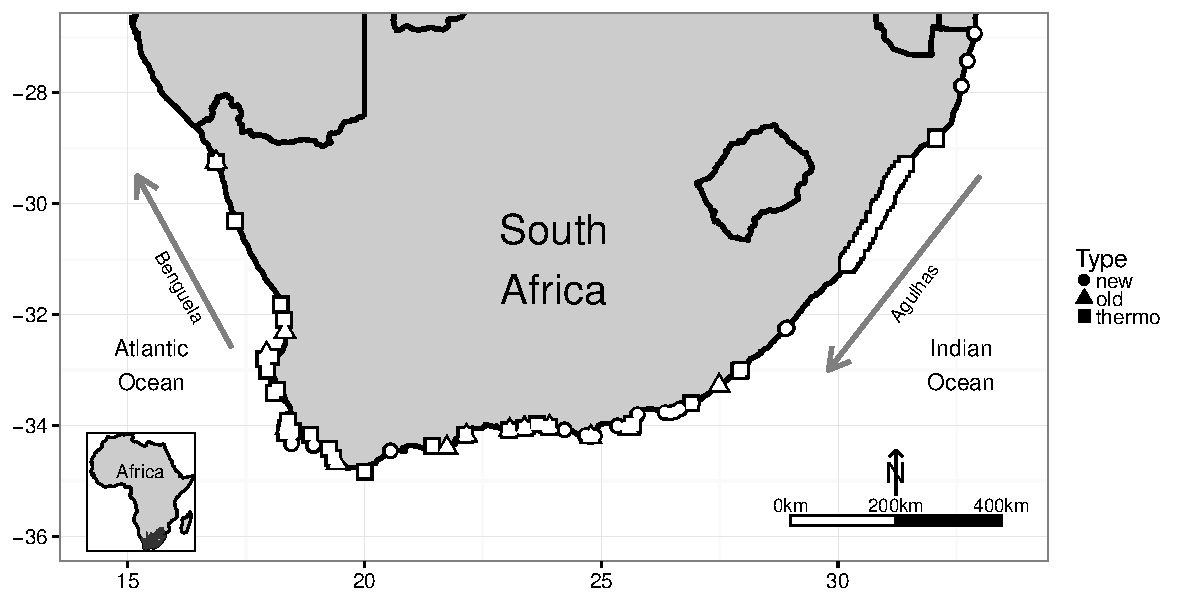
\includegraphics[width=1.0\textwidth]{figure01}
\caption[\small Location and instrument types used to sample each time series available for use in this study]{Location and instrument types used to sample each time series available for use in this study. In the legend, `new' shows the underwater temperature recorder (UTR) time series that were recorded entirely with the newer UTRs that have a high precision of \SI{0.001}{\degreeCelsius}, `old' refers to UTR time series that were recorded, at least in part, with older UTRs and have data with precisions lower than \SI{0.001}{\degreeCelsius}. The `thermo' label shows the location of the thermometer time series.}
\label{figure01}
\end{figure}

\emph{RWS - No longer showing coastal classification.}
% \begin{figure}
% \centering 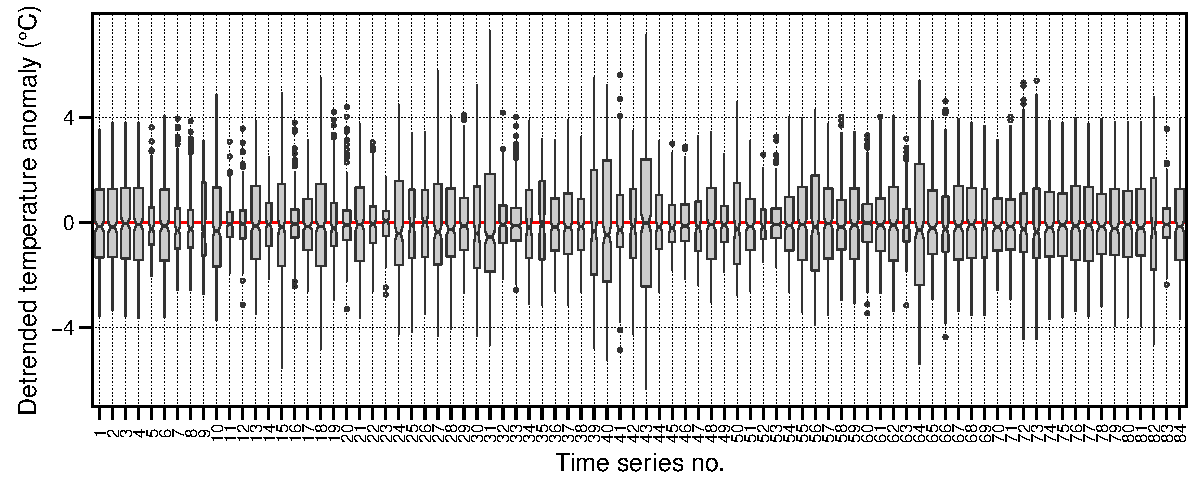
\includegraphics[width=1.0\textwidth]{figure02}
% \caption[\small Coastal allocation of time series from nonmetric multidimensional scaling and hierarchical cluster analysis]{Coastal allocation of time series from nonmetric multidimensional scaling and hierarchical cluster analysis.}
% \label{figure02}
% \end{figure}

\emph{RWS - No longer power analysis results. THis figure could be replaced by a box and whisker plot showing the normal distribution of the data.}
% \begin{figure}
% \centering 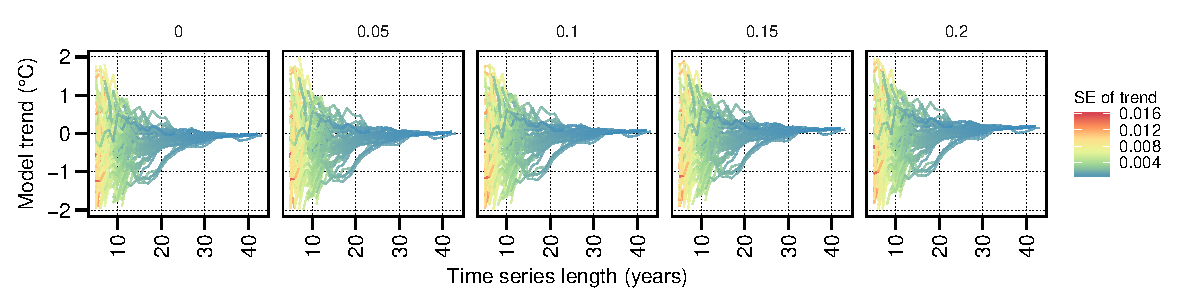
\includegraphics[width=0.66\textwidth]{figure03}
% \caption[\small Boxplots showing the range of lengths required for each subgroup to expect results from a time series analysis with a power of 0.80 or 0.90]{Boxplots showing the range of lengths required for each subgroup to expect results from a time series analysis with a power of 0.80 or 0.90. The median length required for each subgroup is denoted here with thick vertical bars. The ends of the boxplots show the 25th and 75th percentiles. The 95th percentile is shown as text to the left of each boxplot as they distort the range of the \emph{x}-axis. The \emph{n} values listed to the left of each subgroup shows how many time series were drawn on to calculate the statistics for the corresponding boxplots.}
% \label{figure03}
% \end{figure}

\emph{RWS - To be replaced with a new figure.}
% \begin{figure}
% \centering 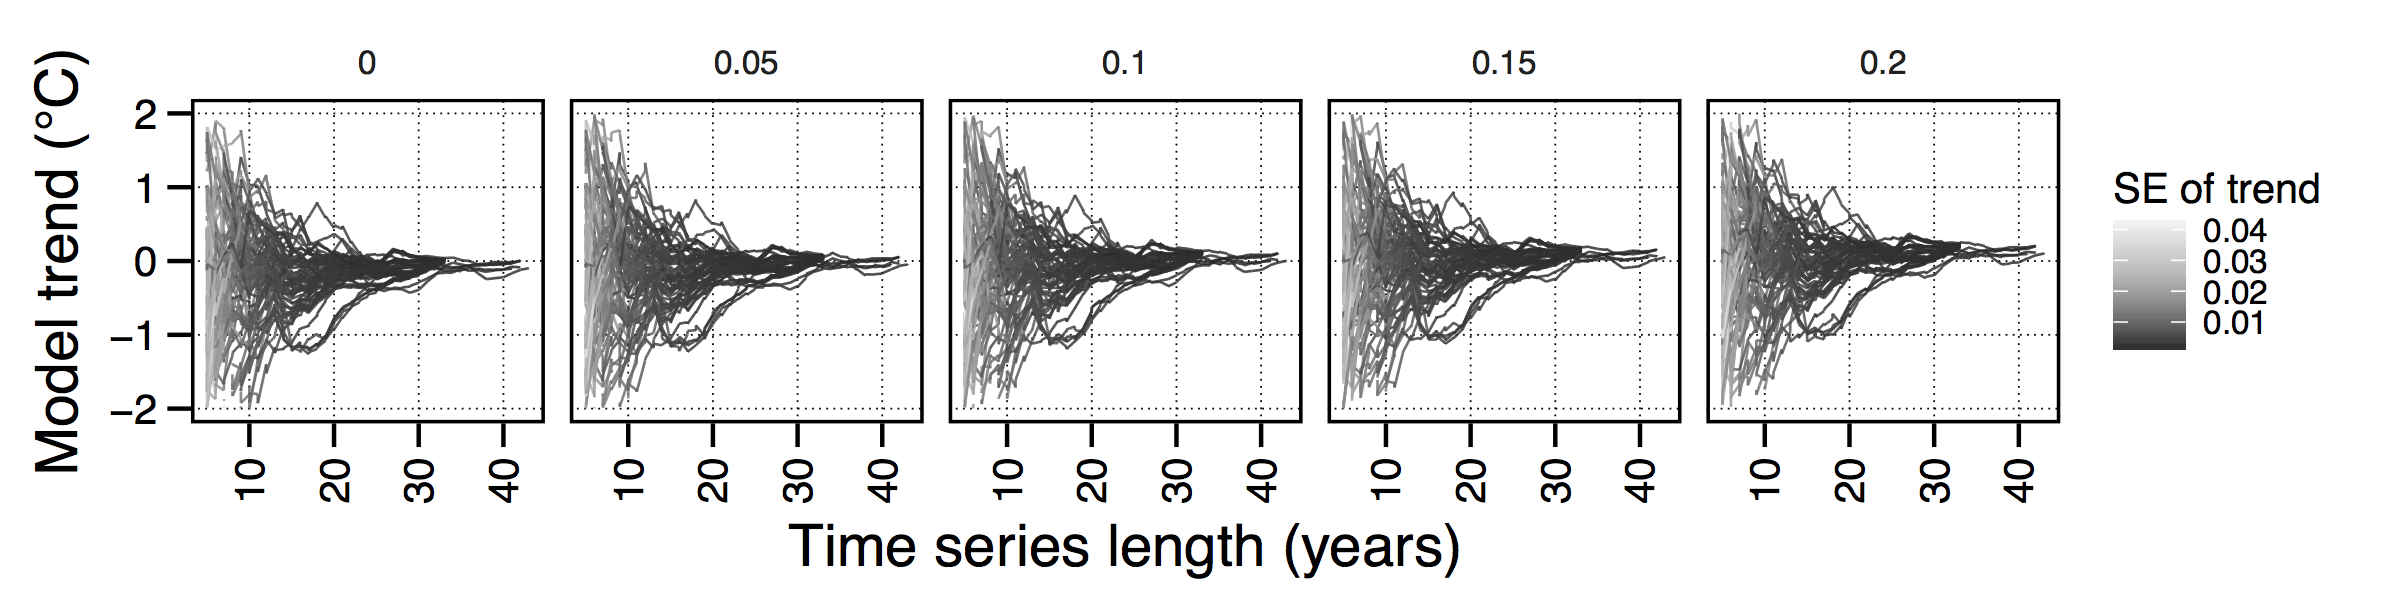
\includegraphics[width=0.66\textwidth]{figure04}
% \caption[\small The effect varying length has on the goodness of fit (\emph{R}\textsuperscript{2}) and significance (\emph{p}) of a linear model fitted to a time time series]{The effect varying length has on the goodness of fit (\emph{R}\textsuperscript{2}) and significance (\emph{p}) of a linear model fitted to a time time series. The number of time series available (\emph{n}) at length 36 months and then for every 60 month interval thereafter for each sub group shown in black in each panel. The median \emph{R}\textsuperscript{2} values are shown as series of dots whose shade shows the median \emph{p} value for that month. \emph{p} values less than 0.05 are shown as black dots, \emph{p} values under 0.10 as grey dots and \emph{p} values greater than 0.10 shown as white dots. The grey ribbon surrounding the dot plot shows the range (5th to 95th percentile) of the \emph{R}\textsuperscript{2} values from each time series for each new month.}
% \label{figure04}
% \end{figure}

\emph{RWS - To be replaced with a new figure.}
% \begin{figure}
% \centering 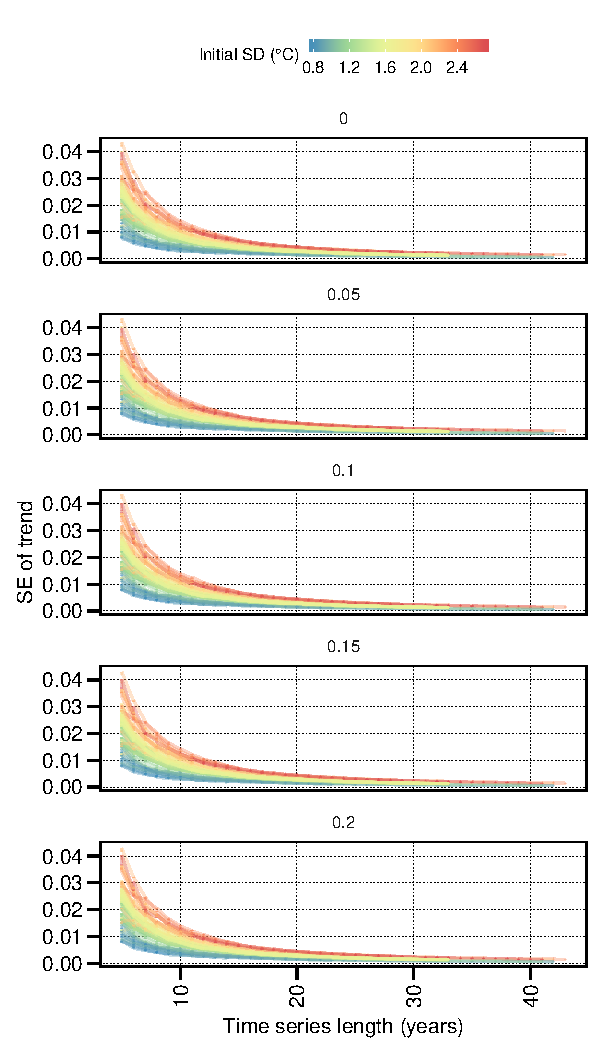
\includegraphics[width=0.66\textwidth]{figure05}
% \caption[\small The effect changes in the SD variable has on the goodness of fit (\emph{R}\textsuperscript{2}) and significance (\emph{p}) of a simple linear model fitted to a time series]{The effect changes in the SD variable has on the goodness of fit (\emph{R}\textsuperscript{2}) and significance (\emph{p}) of a simple linear model fitted to a time series. The number of time series (\emph{n}) used to calculate the effect of varying standard deviation (SD) for each subgroup shown in black in the top right of the corresponding panel. The dots show the median \emph{R}\textsuperscript{2} value for all time series within the corresponding subgroup with the given SD value as seen on the x-axis while the grey ribbon shows the 5th to 95th percentiles for the corresponding point. The colour of each point shows the median \emph{p} value with the same scale as Figure \ref{figure04}.}
% \label{figure05}
% \end{figure}

\end{document}
